\section{Chaining}
This chapter concerns some of the central methods for bounding random processes $(X_t)$. We'll go over concepts 
such as chaining, VC theory, generic chaining methods, and bounds such as Talagrand's inequality and Chevet's 
inequality. We'll apply these to concepts such as Monto Carlo integration, empirical processes, and statistical 
learning theory.



% ----------8.1----------
\subsection{Dudley Inequality}
For a general Gaussian process $(X_t)_{t \in T}$, Sudakove inequality (\cref{thm:7.4.1}) gives a \textit{lower} 
bound on 
\[ \mathbb{E}\left[ \sup_{t \in T}X_t \right] \]
in terms of the metric entropy pf $T$. Now we'll go for an upper bound. Moreover, we generalize from Gaussian 
processes to subgaussian processes as well.

\begin{definition}[]
\label{def:8.1.1}
A random process $(X_t)_{t \in T}$ on a metric space $(T, d)$ has \underline{subgaussian increments} if there 
exists $K > 0$ such that 
\[ \lVert X_t - X_s \rVert_{\psi_2} \leq Kd(t, s) \text{ for all } t, s \in T. \]
\end{definition}

\begin{example}[Gaussian processes]
\label{ex:8.1.2}
Let $(X_t)_{t \in T}$ be a Gaussian process on some set $T$. It naturally defines a \textit{canonical metric} 
on $T$: 
\[ d(t, s) := \lVert X_t - X_s \rVert_{L^2}, \ t, s \in T, \]
as we explained earlier. With respect to this metric, $(X_t)_{t \in T}$ clearly has subgaussian increments, 
with some absolute constant $K$.
\end{example}

Here is another (trivial) example: Any random process can be made to have subgaussian increments by defining 
the metric as $d(t, s) := \lVert X_t - X_s \rVert_{\psi_2}$.

Now we give a bound on a general subgaussian random process in terms of the metric entropy:

\begin{theorem}[Dudley's integral inequality]
\label{thm:8.1.3}
Let $(X_t){t \in T}$ be a mean-zero random process on a metric space $(T, d)$ with subgaussian increments as in 
\cref{def:8.1.1}. Then 
\[ \mathbb{E}\left[ \sup_{t \in T}X_t \right] \leq CK \int_{0}^{\infty} 
\sqrt{\log_{}{\mathcal{N}(T, d, \varepsilon)}} \ d \varepsilon. \]
\end{theorem}

Before going to the proof's let's compare Dudley's inequality with Sudakov's inequality (\cref{thm:7.4.1}), 
which for Gaussian processes, says:
\[ \mathbb{E}\left[ \sup_{t \in T}X_t \right] \geq c \sup_{\varepsilon > 0}\varepsilon 
\sqrt{\log_{}{\mathcal{N}(T, d, \varepsilon)}}. \]
Figure 8.1 below shows both bounds: 
\begin{center}
	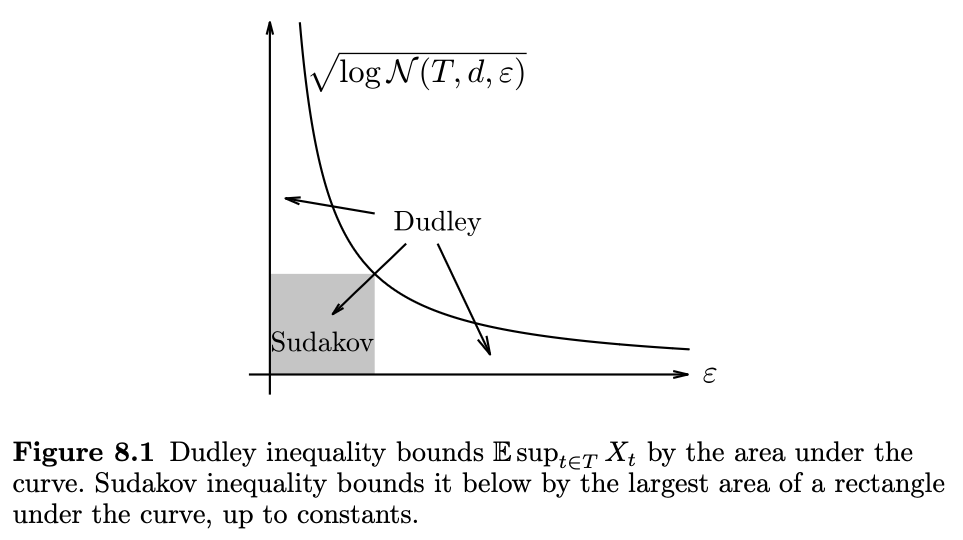
\includegraphics[width=0.8\textwidth]{Chapter 8/fig8-1.png}
\end{center}
There is a clear gap between the two bounds, and it turns out that metric entropy alone cannot close it - we 
will explore this later.

Dudley's inequality hints that $\mathbb{E}\left[ \sup_{t \in T}X_t \right]$ is a \textit{multiscale} quantity 
- to bound it, we need to look at $T$ across all scales $\varepsilon$. That's exactly how the proof works! But 
let's prove a discrete version using syadic scaled $\varepsilon = 2^{-k}$ like a Riemann sum, then move to the 
continuous version later.

\begin{theorem}[Discrete Dudley's inequality]
\label{thm:8.1.4}
Let $(X_t)_{t \in T}$ be a mean-zero random process on a metric space $(T, d)$ with subgaussian increments as 
from earlier. Then 
\[ \mathbb{E}\left[ \sup_{t \in T}X_t \right] \leq CK \sum_{k \in \mathbb{Z}}^{}2^{-k} 
\sqrt{\log_{}{\mathcal{N}(T, d, \varepsilon)}}. \]
\end{theorem}

The proof uses a technique called \textit{chaining}. It is a multi-scaled version of the $\varepsilon$-net 
argument that we did in \cref{thm:4.4.3} and \cref{thm:7.6.1}. In the $\varepsilon$-net argument, we approximate 
$T$ by an $\varepsilon$-net $\mathcal{N}$ so every point $t \in T$ is close to some $\pi(t) \in \mathcal{N}$, 
with $d(t, \pi(t)) \leq \varepsilon$. Then the increment condition gives 
\[ \lVert X_t - X_{\pi(t)} \rVert_{\psi_2} \leq K \varepsilon. \]
This leads to 
\[ \mathbb{E}\left[ \sup_{t \in T}X_t \right] \leq \mathbb{E}\left[ \sup_{t \in T}X_{\pi(t)} \right] 
+ \mathbb{E}\left[ \sup_{t \in T}(X_t - X_{\pi(t)}) \right]. \]
We can handle the first term via union bound over $|\mathcal{N}| = \mathcal{N}(T, d, \varepsilon)$ points 
$\pi(t)$. However, the second term is unclear (if we were to use union bound) since there is both $t$ and 
$\pi(t)$ in the supremum. To fix this, we don't stop at one net, but choose smaller and smaller $\varepsilon$ 
to get better approximations $\pi_1(t), \pi_2(t), \dots$ to $t$ with finer nets. This is the idea behind 
\textit{chaining}.

\begin{proof}[Proof of \cref{thm:8.1.4}]
\textbf{Step 1: Chaining setup.} Without loss of generality, we may assume that $K = 1$ (because of $C$) and 
$T$ is finite (\cref{rmk:7.2.1}). Define the dyadic scale 
\[ \varepsilon_k = 2^{-k}, \ k \in \mathbb{Z} \]
and choose $\varepsilon_k$-nets $T_k$ of $T$ so that 
\[ |T_k| = \mathcal{N}(T, d, \varepsilon_k). \]
Only a part of the dyadic scale will be needed. Since $T$ is finite, there exists a small enough number 
$\kappa \in \mathbb{Z}$ (defining the coarsest net) and a large enough number $K \in \mathbb{Z}$ (defining the 
finest net), such that 
\[ T_{\kappa} = \{t_0\} \text{ for some } t_0 \in T, \ T_K = T. \]
For a point $t \in T$, let $\pi_l(t)$ denote a closest point in $T_k$, so we have 
\[ d(t, \pi_k(t)) \leq \varepsilon_k. \]
Since $\mathbb{E}\left[ X_{t_0} \right] = 0$ by assumption, 
\[ \mathbb{E}\left[ \sup_{x \in T}X_t \right] = \mathbb{E}\left[ \sup_{x \in T}(X_t - X_{t_0}) \right]. \]
Let's write $X_t - X_{t_0}$ as a telescoping sum, walking from $t_0$ to $t$ along a chain (aha!) of points 
$\pi_k(t)$ that mark progressively finer approximations of $t$:
\[ X_t - X_{t_0} = (X_{\pi_{\kappa}(t)} - X_{t_0}) + (X_{\pi_{\kappa + 1}(t)} - X_{\pi_{\kappa}(t)}) 
+ \cdots + (X_t - X_{\pi_{K}(t)}), \]
see Figure 8.2 below for an illustration.
\begin{center}
    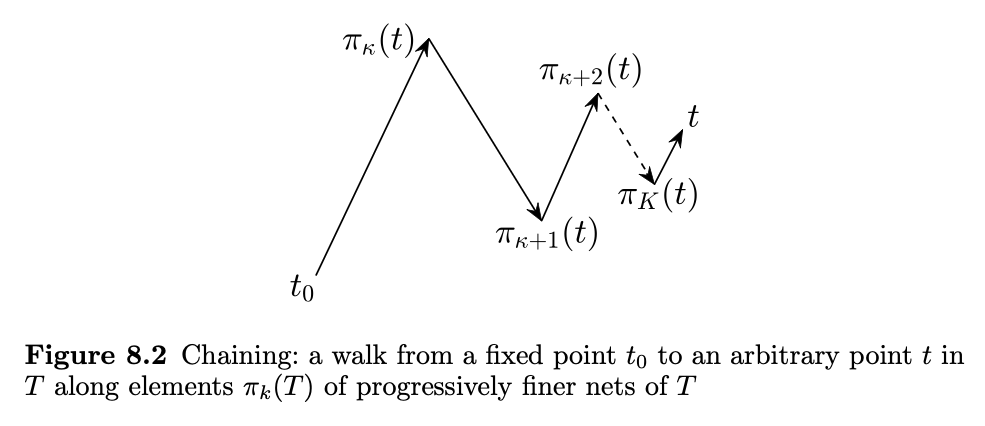
\includegraphics[width=0.8\textwidth]{Chapter 8/fig8-2.png}
\end{center}
The first and last terms of this sum are zero by our definition earlier, so we have 
\[ X_t - X_{t_0} = \sum_{k = \kappa + 1}^{K} (X_{\pi_k(t)} - X_{\pi_{k - 1}(t)}). \]
Since the supremum of the sum is bounded by the sum of the suprema, we get 
\[ \mathbb{E}\left[ \sup_{t \in T}(X_t - X_{t_0}) \right] \leq 
\sum_{k = \kappa + 1}^{K} \mathbb{E}\left[ \sup_{t \in T}(X_{\pi_k(t)} - X_{\pi_{k - 1}(t)}) \right]. \]

\textbf{Step 2: Controlling the increments.} In the equation above, it looks like we are taking the supremum 
over all of $T$ in each summand, but really it is over the smaller set of pairs $(\pi_k(t), \pi_{k - 1}(t))$. 
The number of such pairs is 
\[ |T_k| \cdot |T_{k - 1}| = |T_k|^2, \]
A number that we can control via covering numbers from above. Moreover, for a fixed $t$, we can bound the 
increments in step 1 like this: 
\begin{align*}
	\lVert X_{\pi_k(t)} - X_{\pi_{k - 1}(t)} \rVert_{\psi_2} 
	&\leq d(\pi_k(t), \pi_{k - 1}(t)) \quad \text{(By \cref{def:8.1.1})} \\ 
	&\leq d(\pi_k(t), t) + d(t, \pi_{k - 1}(t)) \quad \text{(By triangle inequality)} \\
	&\leq \varepsilon_k + \varepsilon_{k - 1} \quad \text{(By definition of )} \pi_k(t) \\
	&\leq 2 \varepsilon_{k - 1}.
\end{align*}
Recall from \cref{prop:2.7.6} that the expected maximum of $N$ subgaussian random variables is at most 
$CL \sqrt{\log_{}{N}}$, where $L$ is the largest $\psi_2$ norm. We can use this to bound each term: 
\[ \mathbb{E}\left[ \sup_{t \in T}(X_{\pi_k(t)} - X_{\pi_{k - 1}(t)}) \right] 
\leq C \varepsilon_{k - 1} \sqrt{\log_{}{|T_k|}}. \]

\textbf{Step 3: Summing up the increments.} We have shown that 
\[ \mathbb{E}\left[ \sup_{t \in T}(X_t - X_{t_0}) \right] 
\leq C \sum_{k = \kappa + 1}^{K} \varepsilon_{k - 1} \sqrt{\log_{}{|T_k|}}. \]
Now plug in the values $\varepsilon_k = 2^{-k}$ and the bounds on $|T_k|$, we get 
\[ \mathbb{E}\left[ \sup_{t \in T}(X_t - X_{t_0}) \right] 
\leq C_1 \sum_{k = \kappa + 1}^{K} 2^{-k} \sqrt{\log_{}{\mathcal{N}(T, d, 2^{-k})}}. \]
Hence the theorem is proved.
\end{proof}

Let's now go for the proof for the integral form of Dudley's inequality.

\begin{proof}[Proof of Dudley's integral inequality (\cref{thm:8.1.3})]
To convert the sum from the discrete form into an integral, we express $2^{-k}$ as 
$2 \int_{2^{-k-1}}^{2^{-k}}  \ d \varepsilon$. Then 
\[ \sum_{k \in \mathbb{Z}}^{} 2^{-k} \sqrt{\log_{}{\mathcal{N}(T, d, 2^{-k})}} = 
2 \sum_{k \in \mathbb{Z}}^{} \int_{2^{-k-1}}^{2^{-k}} \sqrt{\log_{}{\mathcal{N}(T, d, 2^{-k})}} \ 
d \varepsilon. \]
Within the limits of the integral, $2^{-k} \geq \varepsilon$, hence $\log_{}{\mathcal{N}(T, d, 2^{-k})} 
< \log_{}{\mathcal{N}(T, d, 2^{-k})}$ and the sum is bounded by 
\[ 2 \sum_{k \in \mathbb{Z}}^{} \int_{2^{-k-1}}^{2^{-k}} \sqrt{\log_{}{\mathcal{N}(T, d, \varepsilon)}} \ 
d \varepsilon = 2 \int_{0}^{\infty} \sqrt{\log_{}{\mathcal{N}(T, d, \varepsilon)}} \ d \varepsilon, \]
and the proof is complete.
\end{proof}

Actually, the discrete and integral Dudley inequalities are equivalent (Exercise 8.3).


\subsubsection{Variations and Examples}
\begin{remark}[Dudley's inequality: supremum of increments]
\label{rmk:8.1.5}
A quick look at the proof shows that chaining actually gives 
\[ \mathbb{E}\left[ \sup_{t \in T}|X_t - X_{t_0}| \right] \leq CK 
\int_{0}^{\infty} \sqrt{\log_{}{\mathcal{N}(T, d, \varepsilon)}} \ d \varepsilon \]
for any fixed $t \in T$. We can combine with the same bound for $X_s - X_{t_0}$, then use the triangle 
inequality to get 
\[ \mathbb{E}\left[ \sup_{t, s \in T}|X_t - X_s| \right] \leq CK 
\int_{0}^{\infty} \sqrt{\log_{}{\mathcal{N}(T, d, \varepsilon)}} \ d \varepsilon. \]
\end{remark}

\begin{remark}[Dudley's inequality: a high-probability bound]
\label{rmk:8.1.6}
Dudley's inequality gives only an expectation bound, but chaining actually gives a high-probability bouind. 
Assuming $T$ is finite (avoid measurability issues), for every $u \geq 0$, the bound 
\[ \sup_{t, s \in T} |X_t - X_s| \leq CK \left[ \int_{0}^{\infty} \sqrt{\log_{}{\mathcal{N}(T, d, \varepsilon)}} 
\ d \varepsilon + u \cdot \mathrm{diam}(T) \right] \]
holds with probability at least $1 - 2 \exp{(-u^2)}$ (Exercise 8.1). For Gaussian processes, this also follows 
directly from Gaussian concentration (Exercise 8.2).
\end{remark}

\begin{remark}[Limits of Dudley integral]
\label{rmk:8.1.7}
Even though the Dudley integral goes over $[0, \infty]$, we can cap it at the diameter of $T$, since for 
$\varepsilon > \mathrm{diam}(T)$, a single $\varepsilon$-ball covers $T$ and so 
\[ \mathcal{N}(T, d, \varepsilon) = 1 \implies \log_{}{\mathcal{N}(T, d, \varepsilon)} = 0. \]
Thus 
\[ \mathbb{E}\left[ \sup_{t \in T}X_t \right] \leq CK \int_{0}^{\mathrm{diam}(T)} 
\sqrt{\log_{}{\mathcal{N}(T, d, \varepsilon)}} \ d \varepsilon. \]
\end{remark}

If we apply Dudley's inequality for the canonical Gaussian process $\left\langle g, t \right\rangle$, just 
like we did with Sudakov's inequality in \cref{cor:7.4.2}, we get the following:

\begin{theorem}[Dudley's inequality in \texorpdfstring{$\mathbb{R}^n$}{}]
\label{thm:8.1.8}
The Gaussian width of any bounded set $Y \subset \mathbb{R}^n$ satisfies 
\[ w(T) \leq C \int_{0}^{\infty} \sqrt{\log_{}{\mathcal{N}(T, \varepsilon)}} \ d \varepsilon, \]
where $\mathcal{N}(T, \varepsilon)$ is the smallest number of Euclidean balls with radius $\varepsilon$ and 
centers in $T$ that cover $T$.
\end{theorem}

\begin{example}[Dudley's inequality is sharp for the Euclidean ball]
\label{ex:8.1.9}
Let's test Dudley's inequality for the unit Euclidean ball $T = B_2^n$. From \cref{cor:4.2.11}, 
\[ \mathcal{N}(B_2^n, \varepsilon) \begin{cases}
	\leq (3 / \varepsilon)^n &\text{ for } \varepsilon \in (0, 1], \\
	= 1 &\text{ for } \varepsilon > 1
\end{cases}. \]
Then 
\[ w(B_2^n) \lesssim \int_{0}^{1} \sqrt{n \log_{}{(3 / \varepsilon)}} \ d \varepsilon \lesssim \sqrt{n}. \]
This is in fact optimal: as we know from \cref{ex:7.5.6}, $w(B_2^n) \asymp \sqrt{n}$.
\end{example}

\begin{remark}[Dudley's inequality can be loose - but not too loose]
\label{rmk:8.1.10}
In general, Dudley integral can overestimate the Gaussian width. Here is a bad example: 
\[ T = \left\{ \frac{e_k}{\sqrt{1 + \log_{}{k}}}, \ k = 1, \dots, n \right\} \]
with $e_k$ being the standard basis in $\mathbb{R}^n$. From exercise 8.4, we can see that 
\[ w(T) = O(1) \text{ while } \int_{0}^{\infty} \sqrt{\log_{}{\mathcal{N}(T, d, \varepsilon)}} \ d \varepsilon 
\to \infty \]
as $n \to \infty$. However, the good news:
\begin{enumerate}
	\item Dudley equality is tight up to a logarithmic factor (Exercise 8.5);
	\item We will use chaining to remove that logarithmic factor in Section 8.5.
\end{enumerate}
\end{remark}


% ----------8.2----------
\subsection{Application: Empirical Processes}
We'll apply Dudley's inequality to \textit{empirical processes} - certain natural random processes indexed by 
functions. Here is a motivating example.


\subsubsection{The Monte Carlo Method}
Suppose we want to compute an integral 
\[ \int_{\Omega}^{} f \ d \mu \]
where $f: \Omega \to \mathbb{R}$ is a given function on some set $\Omega$ and $\mu$ is a probability measure on 
$\Omega$. For instance, this could just be
\[ \int_{0}^{1} f(x) \ dx, \ f: [0, 1] \to \mathbb{R} \]
(See Figure 8.3a).

We can do this \textit{probabilistically}. Suppose $X$ is a random point in $\Omega$ drawn according to $\mu$, 
i.e. $P(X \in A) = \mu(A)$ for any measurable set $A \subset \Omega$. Then the integral becomes the expectation:
\[ \int_{\Omega}^{} f \ d \mu = \mathbb{E}\left[ f(X) \right]. \]
Now take i.i.d. samples $X_1, X_2, \dots$ By the strong law of large numbers (\cref{thm:1.7.1}),
\[ \frac{1}{n}\sum_{i = 1}^{n}f(X_i) \to \mathbb{E}\left[ f(X) \right] \text{ almost surely } \]
as $n \to \infty$. So, we can approximate the integral with just the arithmetic mean:
\[ \int_{\Omega}^{} f \ d \mu \approx \frac{1}{n}\sum_{i = 1}^{n}f(X_i) \]
(See Figure 8.3b). This is the \textit{Monte Carlo Method} - compute the integral by averaging function values 
at random sample points.

\begin{center}
	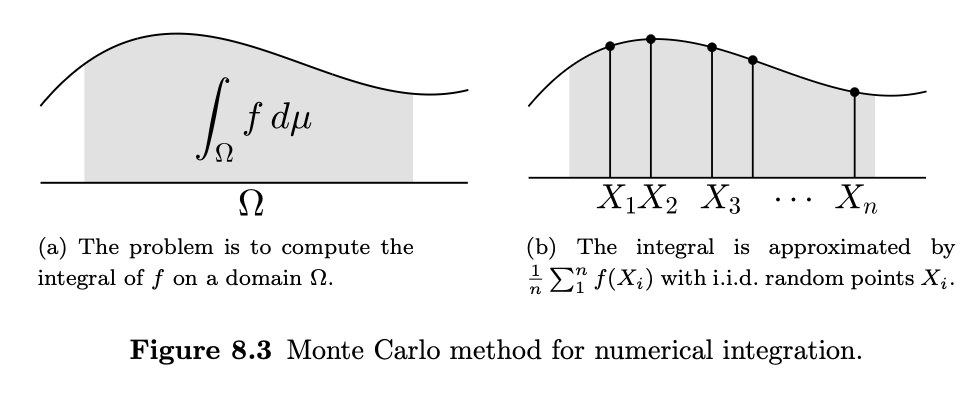
\includegraphics[width=0.8\textwidth]{Chapter 8/fig8-3.png}
\end{center}

\begin{remark}[Error rate]
\label{rmk:8.2.1}
The expected error of the Monte Carlo estimate is $O(1/\sqrt{n})$. This comes from the convergence rate in the 
law of large numbers:
\[ \mathbb{E}\left[ \left| \frac{1}{n}\sum_{i = 1}^{n}f(X_i) - \mathbb{E}\left[ f(X) \right] \right| \right] 
\leq \left[ \mathrm{Var}\left( \frac{1}{n}\sum_{i = 1}^{n}f(X_i) \right) \right]^{1/2} = 
O \left( \frac{1}{\sqrt{n}} \right). \]
\end{remark}

\begin{remark}[Monte Carlo is high-dimensional, agnostic]
\label{rmk:8.2.2}
Monte Carlo works well in high dimensions since the error does not depend on dimension - unlike grid-based 
integration methods. You don't even need to know the measure $\mu$; just being able to sample it is enough. The 
same is with $f$ - you only need its values at just a few points.
\end{remark}


\subsubsection{Lipschitz Law of Large Numbers}
Can we use the same sample $X_1, \dots, X_n$ to estimate the integral of \textit{any} function $f: \Omega \to 
\mathbb{R}$? No. A badly chosen $f$ could wiggle wildly between sample points (Like in Figure 8.4), making the 
Monte Carlo estimate totally off.

\begin{center}
	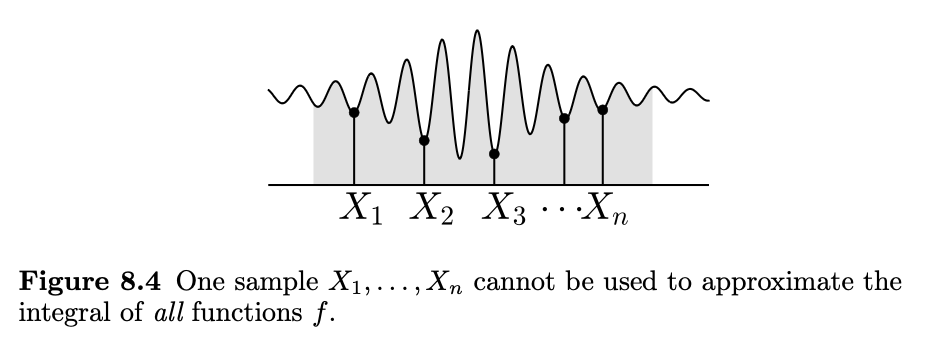
\includegraphics[width=0.8\textwidth]{Chapter 8/fig8-4.png}
\end{center}

But what if we stick to function that don't wiggle too much, like Lipschitz functions? Then yes!

\begin{theorem}[Lipschitz Law of Large Numbers]
\label{thm:8.2.3}
Consider the class of functions 
\[ \mathcal{F} := \{ f: [0, 1] \to \mathbb{R}, \ \lVert f \rVert_{\mathrm{Lip}} \leq L \}, \]
where $L$ is any number. Let $X, X_1, \dots, X_n$ be i.i.d. random variables taking values in $[0, 1]$. Then 
\[ \mathbb{E}\left[ \sup_{f \in \mathcal{F}}\left| \frac{1}{n}\sum_{i = 1}^{n}f(X_i) - 
\mathbb{E}\left[ f(X) \right] \right| \right] \leq \frac{CL}{\sqrt{n}}. \]
\end{theorem}

\begin{remark}[One sample serves all Lipschitz functions]
\label{rmk:8.2.4}
Before the proof, let's iterate the key point: the supremum over $f \in \mathcal{F}$ is \textit{inside} the 
expectation. Thanks to Markov's inequality, this means that a single sample $X_1, \dots, X_n$ will, with high 
probability, work well simultaneously for all $f \in \mathcal{F}$. And ``work well" means approximating each 
integral with $O(1/\sqrt{n})$ error - same rate as the usual law of large numbers with just one function. So, 
we made the law of large numbers uniform without losing anything!
\end{remark}

To make the proof of \cref{thm:8.2.3} more intuitive, we will also introduce empirical processes:
\begin{definition}[]
\label{def:8.2.5}
Let $\mathcal{F}$ be a class of real-valued functions $f: \Omega \to \mathbb{R}$ on some set $\Omega$. Let $X$ 
be a random point in $\Omega$ picked according to some probability distribution, and let $X_1, \dots, X_n$ be 
independent copies of $X$. The random process $(X_f)_{f \in \mathcal{F}}$ defined by 
\[ X_f := \frac{1}{n}\sum_{i = 1}^{n}f(X_i) - \mathbb{E}\left[ f(X) \right] \]
is called an \underline{empirical process} indexed by $\mathcal{F}$m.
\end{definition}

Let's go to the proof!
\begin{proof}[Proof of \cref{thm:8.2.3}]
Without loss of generality, it is enough to prove the theorem for the class
\[ \mathcal{F} := \{ f: [0, 1] \to [0, 1], \lVert f \rVert_{\mathrm{Lip}} \leq 1 \}. \]
We would like to bound 
\[ \mathbb{E}\left[ \sup_{f \in \mathcal{F}}|X_f| \right] \]
for the empirical process $(X_f)_{f \in \mathcal{F}}$ defined earlier.

\textbf{Step 1: Checking subgaussian increments.} Let's use Dudley's inequality (\cref{thm:8.1.3}). To apply 
it, we will check that the empirical process has subgaussian increments with respect to the $L^{\infty}$ metric 
$d(f, g) = \lVert f - g \rVert_{L^\infty}$. So, fix a pair of functions $f, g \in \mathcal{F}$ and write 
\[ \lVert X_f - X_g \rVert_{\psi_2} = \frac{1}{n}\lVert \sum_{i = 1}^{n}Z_i \rVert_{\psi_2} 
\text{ where } Z_i := (f-g)(X_i) - \mathbb{E}\left[ (f-g)(X) \right]. \]
Since $Z_i$ are independent, mean-zero random variables, \cref{prop:2.7.1} gives
\[ \lVert X_f - X_g \rVert_{\psi_2} \lesssim \frac{1}{n}\left( \sum_{i = 1}^{n} 
\lVert Z_i \rVert_{\psi_2}^2 \right)^{1/2}. \]
Now, using centering (\cref{lem:2.7.8}) we have 
\[ \lVert Z_i \rVert_{\psi_2} \lesssim \lVert (f - g)(X_i) \rVert_{\psi_2} \lesssim 
\lVert f - g \rVert_{L^\infty}. \]
It follows that 
\[ \lVert X_f - X_g \rVert_{\psi_2} \lesssim \frac{1}{n} \cdot n^{1/2}\lVert f - g \rVert_{L^\infty} 
= \frac{1}{\sqrt{n}} \lVert f - g \rVert_{L^{\infty}}. \]

\textbf{Step 2: Applying Dudley's inequality.} Now apply Dudley's inequality (\cref{thm:8.1.3}), then we get 
\[ \mathbb{E}\left[ \sup_{f \in \mathcal{F}}|X_f| \right] = 
\mathbb{E}\left[ \sup_{f \in \mathcal{F}}|X_f - X_0| \right] \lesssim 
\frac{1}{\sqrt{n}} \int_{0}^{1} \sqrt{\log_{}{\mathcal{N}(\mathcal{F}, \lVert \cdot \rVert_{L^\infty}, 
\varepsilon)}} \ d \varepsilon. \]
(Here we used that the zero function belongs to $\mathcal{F}$, and the diameter of $\mathcal{F}$ in the 
$L^\infty$ metric is bounded by 1). It is not difficult to bound the covering numbers of $\mathcal{F}$ like 
this (Exercise 8.9):
\[ \mathcal{N}(\mathcal{F}, \lVert \cdot \rVert_{L^\infty}, \varepsilon) \leq e^{C/\varepsilon}. \]
Substitute this bound into the integral, we get 
\[ \mathbb{E}\left[ \sup_{f \in \mathcal{F}}|X_f| \right] \lesssim \frac{1}{\sqrt{n}} 
\int_{0}^{1} \sqrt{\frac{C}{\varepsilon}} \ d \varepsilon \lesssim \frac{1}{\sqrt{n}}. \]
hence the proof is complete.
\end{proof}


\subsubsection{Empirical Measure}
For a broader perspective, take one more look at \cref{def:8.2.5}. Given an i.i.d sample $X_1, \dots, X_n$ 
picked from $\Omega$ according to some probability measure $\mu$, let's consider the \textit{empirical measure} 
$\mu_n$ that assigns equal probabilities $1/n$ to each point, counting multiplicities:
\[ \mu_n = \frac{1}{n}\sum_{i = 1}^{n} \delta_{X_i}. \]
Here $\delta_x$ is the Dirac probability measure at $x$, i.e.
\[ \delta_x(A) = \begin{cases}
	1 &\text{if } x \in A, \\
	0 &\text{otherwise.}
\end{cases} \]
The integral of $f$ with respect to the original measure $\mu$ is $\mathbb{E}\left[ f(X) \right]$, while the 
integral of $f$ with respect to the empirical measure $\mu_n$ is $\frac{1}{n}\sum_{i = 1}^{n}f(X_i)$. The 
empirical process $X_f$ we defined above tracks the deviation of the population expectation from the empirical 
expectation.

This deviation, which we bounded in \cref{thm:8.2.3}, can be thought as a distance between measures $\mu$ and 
$\mu_n$, called the \textit{Wasserstein distance} $W_1(\mu, \mu_n)$. It has an equivalent interpretation as the 
\textit{transportation cost} of turning one measure into the other. The equivalence is provided by the 
Kantorovich-Rubinstein duality theorem. For this reason, \cref{thm:8.2.3} is often called the 
\textit{Wasserstein law of large numbers}.



% ----------8.3----------
\subsection{VC Dimension}
We'll learn about VC dimension, which is a huge part of statistical learning theory. We'll connect it to 
covering numbers, and then, through Dudley's inequality, to random processes and the uniform law of large 
numbers. Applications to statistical learning theory is in the next section.

\subsubsection{Definition and Examples}
VC dimensions measures how complex a class of Boolean functions is, where a Boolean function is a map 
$f: \omega \to \{0, 1\}$ on some set $\omega$, and we are looking at some collection $\mathcal{F}$ of these.

\begin{definition}[]
\label{def:8.3.1}
A subset $\Lambda \subseteq \Omega$ is \underline{shattered} by a class of boolean functions $\mathcal{F}$ if, 
for any possible binary labeling $g: \Lambda \to \{0, 1\}$, there is some function $f \in \mathcal{F}$ that 
matches it on $\Lambda$. Formally, this means the restriction of $f$ onto $\Lambda$ is $g$, i.e. 
$f(x) = g(x) \text{ for all } x \in \Lambda$.

The \underline{Vapnik-Chervonenkis dimension (VC dimension)} of $\mathcal{F}$, denoted 
$\mathrm{vc}(\mathcal{F})$, is the largest cardinality of a subset $\Lambda \subseteq \Omega$ that is shattered. 
If there is no largest one, then $\mathrm{vc}(\mathcal{F}) = \infty$.
\end{definition}

Let's go through a few examples to make the definition clearer:

\begin{example}[Intervals]
\label{ex:8.3.2}
Let $\mathcal{F}$ consist of the indicators of all closed intervals in $\mathbb{R}$:
\[ \mathcal{F} = \left\{ \mathbf{1}_{[a, b]}: \ a, b \in \mathbb{R}, \ a \leq b \right\}. \]
We claim that 
\[ \mathrm{vc}(F) = 2. \]

We first show that $\mathrm{vc}(\mathcal{F}) \geq 2$ by finding a two-point set $\Lambda \subset \mathbb{R}$ 
that is shattered by $\mathcal{F}$. Take, for example, $\Lambda = 3, 5$. There are four possible binary 
labelings $g: \Lambda \to \{0, 1\}$ on this set, and each one can be obtained by restricting some interval 
indicator $f = \mathbf{1}_{[a, b]}$ ontp $\Lambda$. For example, $g(3) = 1, g(5) = 0$ comes from 
$f = \mathbf{1}_{[2, 4]}$. The other three cases are shown in Figure 8.5, so $\Lambda$ is indeed shattered by 
$\mathcal{F}$.

\begin{center}
    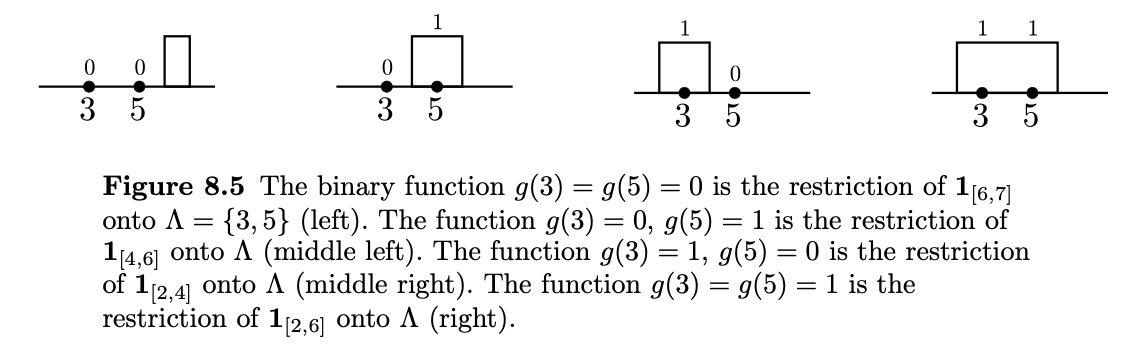
\includegraphics[width=0.8\textwidth]{Chapter 8/fig8-5.png}
\end{center}

To prove $\mathrm{vc}(\mathcal{F}) < 3$, we need to show that no three-point set $\Lambda = \{p, q, r\}$ can 
be shattered by $\mathcal{F}$. To see this, assume $p < q < r$ and consider the labeling $g(p) = 1, g(q) = 0, 
g(r) = 1$. Then $g$ cannot be a restriction of any indicator interval onto $\Lambda$ (it is not linearly 
seperable).
\end{example}

\begin{example}[Half-planes]
\label{ex:8.3.3}
Let $\mathcal{f}$ consist of the indicators of all closed half-planes in $\mathbb{R}^2$. Then we claim that 
\[ \mathrm{vc}(\mathcal{F}) = 3. \]
To prove $\mathrm{vc}(\mathcal{F}) \geq 3$, we need to find a three-point set $\Lambda \subset \mathbb{R}^2$ 
that is shattered by $\mathcal{F}$. Let $\Lambda$ consist of three points in general posiition like in Figure 
8.6 below. Each of the $2^3 = 8$ binary labelings $g: \Lambda \to \{0, 1\}$ is a restriction of the indicator 
function of some half-plane. Too see this, attange the half-plane to containe exactly these points where $g$ 
takes value $1$. Thus, $\Lambda$ is shattered.

\begin{center}
    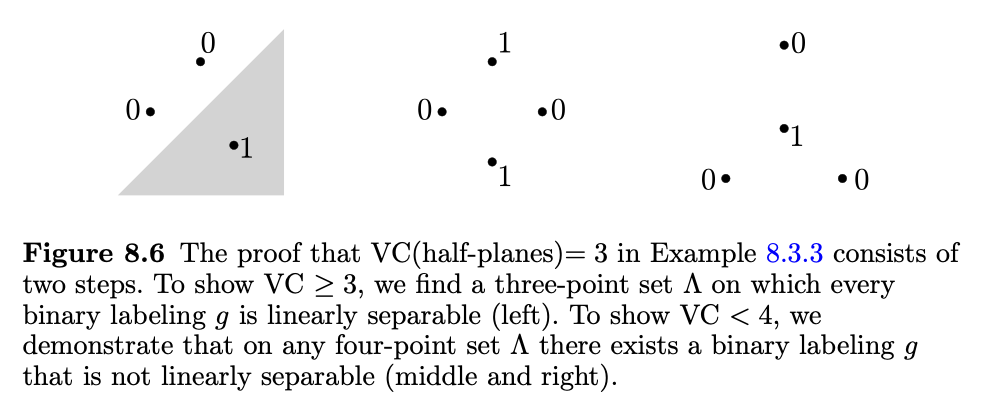
\includegraphics[width=0.8\textwidth]{Chapter 8/fig8-6.png}
\end{center}

To prove $\mathrm{vc}(\mathcal{F}) < 4$, we need to show that no four-point set can be shattered by 
$\mathcal{F}$. There are two possible configurations of four-point sets $\Lambda$ in general position, shown 
also in Figure 8.6. In each of the two cases, there exists a binary labeling such that no half-plane can contain 
exactly the points labeled 1. This means that there always exists a binary labeling $g: \Lambda \to \{0, 1\}$ 
that is not a restriction of any indicator of a half-plane, and thus $\Lambda$ is not shattered.
\end{example}

\begin{example}[]
\label{ex:8.3.4}
Let $\Omega = \{1, 2, 3\}$. We can conveniently represent Boolean functions on $\Omega$ as binary strings of 
length three. Consider the class 
\[ \mathcal{F} = \{001, 010, 100, 111\}. \]
The set $\Lambda = \{1, 3\}$ is shattered by $\mathcal{F}$. Indeed, restricting the functions in $\mathcal{F}$ 
onto $\Lambda$ amounts to dropping the second digit, thus producing the strings 00, 01, 10, 11. Thys, the 
restriction produces all possible binary strings of length two, or equivalently, all possible binary labelings 
$g: \Lambda \to \{0, 1\}$. Hence $\Lambda$ is shattered by $\mathcal{F}$, and thus 
\[ \mathrm{vc}(\mathcal{F}) \geq |\Lambda| = 2. \]
On the other hand, the (only) three-point set $\{1, 2, 3\}$ is not shattered by $\mathcal{F}$, as that would 
require all eight binary digits of length three to appear in $\mathcal{F}$, which is not true.
\end{example}

\begin{example}[Half-spaces]
\label{ex:8.3.5}
A half-space in $\mathbb{R}^m$ is a set of the form 
\[ \{x: \ \left\langle a, x \right\rangle \leq b\} \text{ where } a \in \mathbb{R}^n \text{ and } b 
\in \mathbb{R}. \]
Let $\mathcal{F}$ be the class of indicators of all half-spaces in $\mathbb{R}^n$. Then 
\[ \mathrm{vc}(\mathcal{F}) = n + 1. \]
\end{example}

\begin{remark}[VC dimension v.s. parameter count]
\label{rmk:8.3.6}
The VC dimension of a function class often roughly matches the number of parameters - for instance, half-spaces 
in $\mathbb{R}^n$ are defined with $n + 1$ parameters, which matches the VC dimensions (\cref{ex:8.3.5}). This 
is not a hard rule but rather a useful heuristic.
\end{remark}


\subsubsection{Pajor's Lemma}
Suppose the domain $\Omega$ is finite and consists of $n$ points. Then any class of Boolean functions 
$\mathcal{F}$ on $\Omega$ is also finite, and 
\[ 2^{\mathrm{vc}(\mathcal{F})} \leq |\mathcal{F}| \leq 2^n. \]
The upper bound is usually loose - most function classes are closer in side to the lower bound. This is not so 
obvious. To prepare for this result, let's first show that there are as many shattered subsets of $\Omega$ as 
the functions in $\mathcal{F}$.

\begin{lemma}[Pajor's lemma]
\label{lem:8.3.7}
Let $\mathcal{F}$ be a class of Boolearn functions on a finite set $\Omega$. Then 
\[ |\mathcal{F}| \leq |\{ \Lambda \subseteq \Omega: \ \Lambda \text{ is shattered by } \mathcal{F} \}|. \]
We include the empty set $\Lambda = \emptyset$ in the count on the right side.
\end{lemma}

Before the proof, let's illustrate this result using \cref{ex:8.3.4}. Here, $|\mathcal{F}| = 4$ and there are 
six subsets $\Lambda$ that are shattered by $\mathcal{F}$, namely $\{1\}, \{2\}, \{3\}, \{1, 2\}, \{1, 3\}$, 
and $\{2, 3\}$. Thus the inequalty in Pajor's lemma reads $4 \leq 6$.

\begin{proof}[Proof of \cref{lem:8.3.7}]
We proceed by induction on the cardinality of $\Omega$. The case $|\Omega| = 1$ is trivial, since we include the 
empty set in the counting. 

For the inductive step, assume the lemma holds for any $n$-point set $\Omega$. Now look at a set $\Omega$ with 
$|\Omega| = n + 1$. Chopping out one (arbitrary) point from the set $\Omega$, we can express it as 
\[ \Omega = \Omega_0 \cup \{x_0\}, \text{ where } |\Omega_0| = n. \]
The class $\mathcal{F}$ then natually breaks into two subclasses 
\[ \mathcal{F}_0 := \{ f \in \mathcal{F}: \ f(x_0) = 0 \} \text{ and } 
\mathcal{F}_1 := \{ f \in \mathcal{F}: \ f(x_0) = 1 \}. \]
By the induction hypothesis, the counting function 
\[ S(\mathcal{F}) = |\{ \Lambda \subseteq \Omega: \ \Lambda \text{ is shattered by } \mathcal{F} \}| \]
satisfies (by restricting to $\Omega_0$)
\[ S(\mathcal{F}_0) \geq |\mathcal{F}_0| \text{ and } S(\mathcal{F}_1) \geq |\mathcal{F}_1|. \]

To complete the proof, all we need to check is 
\[ S(\mathcal{F}) \geq S(\mathcal{F}_0) + S(\mathcal{F}_1), \]
for then the inductive hypothesis would give $S(\mathcal{F}) \geq |\mathcal{F}_0| + |\mathcal{F}_1|
= |\mathcal{F}|$, as needed.

The inequality above may seem trivial. Any set $\Lambda$ that is shattered by $\mathcal{F}_0$ or $\mathcal{F}_1$ 
is automatically shattered by the larger class $\mathcal{F}$, and thus each set $\Lambda$ counted by 
$S(\mathcal{F}_0)$ or $S(\mathcal{F}_1)$ is automatically counted by $S(\mathcal{F})$. However, there may be 
the risk of double counting. Assume the same set $\Lambda$ is shattered by both $\mathcal{F}_0$ and 
$\mathcal{F}_1$. The counting function $S(\mathcal{F})$ will not count $\Lambda$ twice. However, a different set 
will be counted by $S(\mathcal{F})$, which was not counted by either $S_(\mathcal{F}_0)$ or $S(\mathcal{F}_1)$ - 
namely, $\Lambda \cup \{x_0\}$. This set is indeed shattered by $\mathcal{F}$. This establishes the inequality 
above, and the proof is complete.
\end{proof}

Let's illustrate the proof above via an example: 
\begin{example}[]
\label{ex:8.3.8}
Let's reuse \cref{ex:8.3.4}. Following the proof of Pajor's lemma, we chop out $x_0 = 3$ from $\Omega = \{1, 
2, 3\}$, making $\Omega_0 = \{1, 2\}$. The class $\mathcal{F} = \{001, 010, 100, 111\}$ then breaks into two 
sub-classes
\[ \mathcal{F}_0 = \{010, 100\} \text{ and } \mathcal{F}_1 = \{001, 111\}. \]
There are exactly two subsets $\Lambda$ shattered by $\mathcal{F}_0$, namely $\{1\}$ and $\{2\}$, and the same 
two subsets are shattered by $\mathcal{F}_1$, making $S(\mathcal{F}_0) = S(\mathcal{F}_1) = 2$. Of course, the 
same two subsets are also shattered by $\mathcal{F}$, but we need two more shattered subsets to make 
$S(\mathcal{F}) \geq 4$ for the key inequality. Here is how we construct them:

Append $x_0 = 3$ to the already counted subsets $\Lambda$. The resulting sets $\{1, 3\}$ and $\{2, 3\}$ are 
also shattered by $\mathcal{F}$, and we have not counted them yet. Now we have at least four subsets shattered 
by $\mathcal{F}$, making the inequality in Pajor's lemma true.
\end{example}


\subsubsection{Sauer-Shelah Lemma}
We now deduce a remarkable upper bound on the cardinality of a function class in terms of the VC dimension:

\begin{lemma}[Sauer-Shelah lemma]
\label{lem:8.3.9}
Let $\mathcal{F}$ be a class of Boolean functions on an $n$-point set $\Omega$. Then 
\[ |\mathcal{F}| \leq \sum_{k = 0}^{d} \binom{n}{k} \leq \left( \frac{en}{d} \right)^d \text{ where } 
d = \mathrm{vc}(\mathcal{F}). \]
\end{lemma}

\begin{proof}
Pajor's lemma states that $|\mathcal{F}|$ is bounded by the number of subsets $\Lambda \subseteq \Omega$ 
shattered by $\mathcal{F}$. The cardinality of each such set $\Lambda$ is bounded by $d = 
\mathrm{vc}(\mathcal{F})$, via the definition of VC dimension (\cref{def:8.3.1}). Thus 
\[ |\mathcal{F}| \leq |\{ \Lambda \subseteq \Omega: \ |\Lambda| \leq d \}| 
= \sum_{k = 0}^{d} \binom{n}{k} \]
since the sum oin the right hand side gives the total number of subsets of an $n$-elements set with 
cardinalities at most $k$. This proces the first inequality of the Sauer-Shelah lemma. The second inequality 
follows from the bound on the binomial sum from Exercise 0.6. The proof is complete.
\end{proof}

Both Pajor's and Sauer-Shelah lemma are generally sharp (Exercise 8.19).


\subsubsection{Growth Function}
The Sauer-Shelah lemma assumes that the domain $\Omega$ is finite. What if the function classes $\mathcal{F}$ 
are on infinite domains like $\mathbb{R}^n$? It is often convenient to measure the complexity of $\mathcal{F}$ 
by the growth function:

\begin{definition}[]
\label{def:8.3.10}
Let $\mathcal{F}$ be a class of Boolean functions on a domain $\Omega$. The \underline{growth function} of 
$\mathcal{F}$ is defined as the maximum number of functions that can be obtained by restricting all functions in 
$\mathcal{F}$ to a subset of $n$ elements: 
\[ \Pi_{\mathcal{F}}(n) = \sup_{} \left\{ \left| \mathcal{F}|_{\Lambda} \right| : \ \Lambda \subset \Omega, 
\ |\Lambda| = n \right\}. \]
\end{definition}

In this light, the VC dimension of $\mathcal{F}$ can be seen as the largest $d$ for which $\Pi_{\mathcal{F}}(d) 
= 2^d$. Immediate bounds on the growth function are 
\[ 2^d \leq \Pi_{\mathcal{F}}(n) \leq \left( \frac{en}{d} \right)^d \text{ for all } n \geq d \]
if $d = \mathrm{vc}(\mathcal{F}) < \infty$. The lower bound is a restatement from the part before Pajor's lemma, 
and the upper bound follows from the Sauer-Shelah lemma (\cref{lem:8.3.9}).

To see how the growth function can be useful, let's duduce from above the stability of VC dimension with 
respect to natural operations.

\begin{proposition}[VC stability]
\label{prop:8.3.11}
Let $\mathcal{F}, \mathcal{G}$ be two classes of Boolean functions on the same domain. Let 
\[ \mathcal{F} \wedge \mathcal{G} = \{ f \wedge g: \ f \in F, \ g \in G \} \]
where $f \wedge g$ denotes the pointwise minimum of the functions $f$ and $g$. Then 
\[ \mathrm{vc}(\mathcal{F} \wedge \mathcal{G}) \leq 10 \max_{}(\mathrm{vc}(\mathcal{F}), 
\mathrm{vc}(\mathcal{G})). \]
The same holds for the pointwise maximum.
\end{proposition}

\begin{proof}
Assume towards a contradiction that $n := \mathrm{vc}(\mathcal{F} \wedge \mathcal{G}) > 10d$. Then 
\[ 2^n \leq \Pi_{\mathcal{F} \wedge \mathcal{G}}(n) \leq \Pi_{\mathcal{F}}(n) \cdot \Pi_{\mathcal{G}}(n) 
\leq \left( \frac{en}{d} \right)^{2d}. \]
The first and last bounds directly follow from the bounds of the growth function above, and the middle one is 
true by definition. However, we can calculate and show that $2^n > (en / d)^{2d}$ whenever $n > 10d$, which 
is a contradiction to the above.
\end{proof}

\cref{prop:8.3.11} can be extended to any particular way of combining classes of functions (Exercise 8.21). It 
can be helpful when we want to bound the VC dimension without computing it directly (which can be quite 
complicated). For example:

\begin{example}[Strips]
\label{ex:8.3.12}
A strip in $\mathbb{R}^n$ is a set of the form 
\[ \{ x: \ |\left\langle a, x \right\rangle - b| \leq c \} \text{ where } a \in \mathbb{R}^n \text{ and } 
b, c \in \mathbb{R}. \]
For an illustration, see Figure 8.7 below: 
\begin{center}
    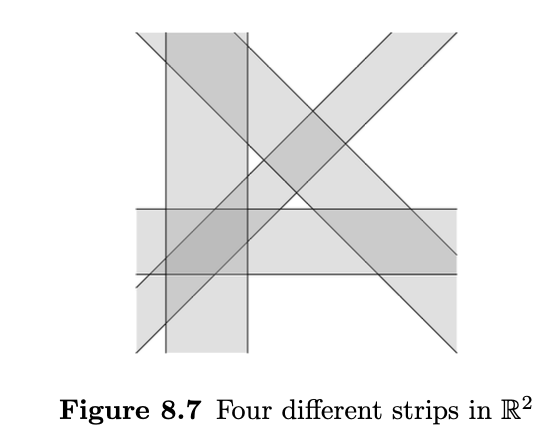
\includegraphics[width=0.8\textwidth]{Chapter 8/fig8-7.png}
\end{center}

Let $\mathcal{F}$ be the class of indicators of strips. \cref{ex:8.3.5} gives 
\[ \mathrm{vc}(\mathcal{F}) \leq 20(n + 1) \leq 40n. \]
Indeed, each strip can be represented as the intersection of two half planes $\{ x: \ \left\langle a, x
\right\rangle - b \leq c \}$ and $\{ x: \ \left\langle a, x \right\rangle - b \geq -c \}$. Thus the indicator of 
each strip is the pointwise mimimum of the indicators of two hald-spaces. Now apply the VC stability property 
(\cref{prop:8.3.11}) and the result in \cref{ex:8.3.5} to get the bound above. 
\end{example}


\subsubsection{Covering Numbers via VC Dimension}
Covering numbers usually grow exponentially with dimension. Now, let's refine this heuristic by replacing the 
algebraic dimension with the VC dimension - which can save us a lot.

Let $\mathcal{F}$ be a class of Boolean functions on some domain $\Omega$, and let $\mu$ be any probability 
measure on $\Omega$. Define the distance between functions as 
\[ d(f, g) = \lVert f - g \rVert_{L^2(\mu)} = \left( \mathbb{E}\left[ (f - g)(X)^2 \right] \right)^{1/2} \]
where $X$ is a random variable with distribution $\mu$. Now let's bound the covering numbers 
$\mathcal{N}(\mathcal{F}, L^2(\mu), \varepsilon)$ of the class $\mathcal{F}$ with respect to the metric above:

\begin{theorem}[Covering numbers via VC dimension]
\label{thm:8.3.13}
Let $\mathcal{F}$ be a class of Boolean functions on a domain $\Omega$ with a probability measure $\mu$ on it. 
Then, for every $\varepsilon \in (0, 1)$, 
\[ \mathcal{N}(\mathcal{F}, L^2(\mu), \varepsilon0) \leq \left( \frac{2}{\varepsilon} \right)^{Cd} 
\text{ where } d = \mathrm{vc}(\mathcal{F}). \]
\end{theorem}

For a first attempt of the proof, let's assume for a moment that $\Omega$ is finite, say $|\Omega| = n$. 
Then the Sauer-Shelah lemma (\cref{lem:8.3.9}) gives 
\[ \mathcal{N}(\mathcal{F}, L^2(\mu), \varepsilon) \leq |\mathcal{F}| \leq \left( \frac{en}{d} \right)^d. \]
This not quite the result above, but it comes close. To tighten the bound, we need to get rid of $n$, and 
we'll do this by shrinking $\Omega$. This lemma would help: 

\begin{lemma}[Dimension reduction]
\label{lem:8.3.14}
Let $\mathcal{F}$ be a finite class of Boolean functions on a domain $\Omega$ with a probability measure $\mu$ 
on it. Assume that all functions in $\mathcal{F}$ are $\varepsilon$-seperated, i.e.
\[ \lVert f - g \rVert_{L^2(\mu)} > \varepsilon \text{ for all distinct } f, g \in \mathcal{F}. \]
IF $n \geq C \varepsilon^{-4}\log_{}{|F|}$, then the empirical measure $\mu_n$ satisfies the following with 
probability at least 0.99:
\[ \lVert f - g \rVert_{L^2(\mu_n)} > \varepsilon / 2 \text{ for all distinct } f, g \in \mathcal{F}. \]
\end{lemma}

By definition of the empirical measure, $\lVert f - g \rVert_{L^2(\mu_n)}$ is the same as the metric we defined 
in the beginning of this subsection, but with the population average replaced by the sample average:
\[ \lVert f - g \rVert_{L^2(\mu_n)} = \left( \frac{1}{n}\sum_{i = 1}^{n}(f - g)(X_i)^2 \right)^{1/2}, \]
where $X_i$ are i.i.d. copies of $X$.


\begin{proof}[Proof of \cref{lem:8.3.14}]
The proof is like that of the Johnson-Lindenstrauss lemma - concentration plus a union bound.

Fix a pair of distinct functions $f, g \in \mathcal{F}$, and consider 
\[ \lVert f - g \rVert_{L^2(\mu_n)}^2 - \lVert f - g \rVert_{L^2(\mu)}^2 
= \frac{1}{n}\sum_{i = 1}^{n} h(X_i) - \mathbb{E}\left[ h(X) \right], \]
where $h = (f - g)^2$. On the right, we have a sum of independent bounded (and thus subgaussian) random 
variables, so Hoeffding inequality (\cref{thm:2.7.3}) gives 
\[ P \left( \left| \lVert f - g \rVert_{L^2(\mu_n)}^2 - \lVert f - g \rVert_{L^2(\mu)}^2 \right) \right| 
> \frac{\varepsilon^2}{4} \right) \leq 2 \exp{(-cn \varepsilon^4)}. \]
Therefore, with probability at least $1 - 2 \exp{(-cn \varepsilon^4)}$, we have 
\[ \lVert f - g \rVert_{L^2(\mu_n)}^2 \geq \lVert f - g \rVert_{L^2(\mu)}^2 - \frac{\varepsilon^2}{4} 
> \varepsilon^2 - \frac{\varepsilon^2}{4} > \frac{\varepsilon^2}{4}, \]
by the lemma's assumption. Now, take a union bound over all pairs of distinct functions $f, g \in \mathcal{F}$. 
There are at most $|\mathcal{F}|^2$ of them, so with probability at least 
\[ 1 - |\mathcal{F}|^2 \cdot 2 \exp{(-cn \varepsilon^4)}, \]
the bound holds simultaneously for all distinct $f, g \in \mathcal{F}$. By out choise of $n$, choosing a large 
enough $C$ yields the quantity above at least 0.99. The proof is complete.
\end{proof}

\begin{proof}[Proof of \cref{thm:8.3.13}]
By the packing-covering equivalence (\cref{lem:4.2.8}), we can find 
\[ N = \mathcal{N}(\mathcal{F}, L^2(\mu), \varepsilon) \]
functions in $\mathcal{F}$ that are $\varepsilon$-seperated in the $L^2(\mu)$ metric. Set $n = \left\lfloor C 
\varepsilon^{-4} \log_{}{N} \right\rfloor$ and apply \cref{lem:8.3.14} to the set of those functions. With 
positive probability, those functions stay $(\varepsilon / 2)$-seperated in the metric $L^2(\mu_n)$ defined 
earlier, so their restrictions onto $\Omega_n = \{ X_1, \dots, X_n \}$ are all different.

Fix a realization of random variables $X_1, \dots, X_n$ for which the event holds. So there exists a subset 
$\Omega_n \subset \Omega$ with $\Omega_n \leq n \leq 2C \varepsilon^{-4} \log_{}{N}$, such that the class 
$\mathcal{F}_n = \mathcal{F}|_{\Omega_n}$ obtained by restricting all functions onto $\Omega_n$ satisfies 
$|\mathcal{F}_n| \geq N$. Now apply the Sauer-Shelah lemma (\cref{lem:8.3.9}) for $\mathcal{F}_n$ and 
$\Omega_n$ to get 
\[ N \leq \left( \frac{en}{d_n} \right)^{d_n} \leq \left( \frac{2C \varepsilon^{-4} \log_{}{N}}{d_n} 
\right)^{d_n} \]
where $d_n = \mathrm{vc}(\mathcal{F}_n)$. Simplifying, we get 
\[ N \leq (2C \varepsilon^{-4})^{2d_n}. \]
Finally, replace $d_n = \mathrm{vc}(\mathcal{F}_n)$ by the larger quantity $d = \mathrm{vc}(\mathcal{F})$ and 
the proof is complete.
\end{proof}


\subsubsection{VC Law of Large Numbers}
Any class of Boolean functions with finite VC dimension has a LLN property: 

\begin{theorem}[VC law of large numbers]
\label{thm:8.3.15}
Let $\mathcal{F}$ be a class of Boolean functions with finite VC dimension on some domain $\Omega$, and let 
$X, X_1, X_2, \dots, X_n$ be independent random points in $\Omega$ with common distribution. Then 
\[ \mathbb{E}\left[ \sup_{f \in \mathcal{F}} \left| \frac{1}{n}\sum_{i = 1}^{n} f(X_i) - \mathbb{E}\left[ f(X) 
\right] \right| \right] \leq C \sqrt{\frac{\mathrm{vc}(\mathcal{F})}{n}}. \]
\end{theorem}

\begin{proof}
We will combine Dudley's inequality with the bound on the covering numbers (\cref{thm:8.3.13}). But first, 
let's symmetrize the process using the empirical version of symmetrization (Exercise 8.11):
\[ \mathbb{E}\left[ \sup_{f \in \mathcal{F}} \left| \frac{1}{n}\sum_{i = 1}^{n} f(X_i) - \mathbb{E}\left[ f(X) 
\right] \right| \right] \leq \frac{2}{\sqrt{n}} \mathbb{E}\left[ \sup_{f \in \mathcal{F}} 
\underbrace{\left| \frac{1}{\sqrt{n}}\sum_{i = 1}^{n} \varepsilon_i f(X_i) \right|}_{Z_f} \right]. \]
Condition on $(X_i)$, leaving all randomness in the random signs $(\varepsilon)_i$. To use Dudley's inequality 
for the process $(Z_f)_{f \in \mathcal{F}}$, we need to check that the increments are subgaussian. Triangle 
inequality gives 
\[ |Z_f - Z_g| \leq \frac{1}{\sqrt{n}} \left| \sum_{i = 1}^{n} \varepsilon_i(f - g)(X_i) \right|, \]
so using \cref{prop:2.7.1} and the fact that $\lVert \varepsilon_i \rVert_{\psi_2} \lesssim 1$, we get:
\begin{align*}
	\lVert Z_f - Z_g \rVert_{\psi_2} 
	&\leq \frac{1}{\sqrt{n}} \left\lVert \sum_{i = 1}^{n} \varepsilon_i(f - g)(X_i) \right\rVert_{\psi_2} \\
	&\lesssim \left( \frac{1}{n} \sum_{i = 1}^{n} (f - g)(X_i)^2 \right)^{1/2} \\
	&= \lVert f - g \rVert_{L^2(\mu_n)}
\end{align*}
where $\mu_n$ is the empirical measure, as mentioned before.

Now use Dudley's inequality (\cref{thm:8.1.3}) conditionallyh on $(X_i)$, then remove the conditioning by taking 
expectation with respect to $(X_i)$. Check that $\mathrm{diam}(\mathcal{F}) \leq 1$. We get 
\[ \frac{2}{\sqrt{n}} \mathbb{E}\left[ \sup_{f \in \mathcal{F}} Z_f \right] \lesssim 
\frac{1}{\sqrt{n}} \mathbb{E}\left[ \int_{0}^{1} \sqrt{\log_{}{\mathcal{N}(\mathcal{F}, L^2(\mu_n), 
\varepsilon)}} \ d \varepsilon \right]. \]
Finally, we use \cref{thm:8.3.13} to bound the covering numbers:
\[ \log_{}{\mathcal{N}(\mathcal{F}, L^2(\mu_n), \varepsilon)} \lesssim \mathrm{vc}(\mathcal{F}) 
\log_{}{(2 / \varepsilon)}. \]
Substituting this into the bound above, we get the integral of $\sqrt{\log_{}{(2 / \varepsilon)}}$, which is 
bounded by an absolute constant, leading to 
\[ \frac{2}{\sqrt{n}} \mathbb{E}\left[ \sup_{f \in \mathcal{F}}Z_f \right] \lesssim 
\sqrt{\frac{\mathrm{vc}(\mathcal{F})}{n}}, \]
hence the proof is complete.
\end{proof}

\begin{remark}[Rademacher complexity]
\label{rmk:8.3.16}
If $\mathcal{F}$ is a class of Boolean functions with finite VC dimension, then the expression 
\[ \mathbb{E}\left[ \sup_{f \in \mathcal{F}} \left| \frac{1}{n}\sum_{i = 1}^{n} \varepsilon_i f(x_i) \right|
\right]\]
is called the \textit{Rademacher complexity} of $\mathcal{F}$ on a given set of points $x_1, \dots, x_n \in 
\Omega$. Rademacher complexity reflects how rich $\mathcal{F}$ is. In proving \cref{thm:8.3.15}, a key step 
was relating it to another measure of richness - the VC dimension: we showed that the Rademacher complexity of 
$\mathcal{F}$ is bounded by $C \sqrt{\mathrm{vc}(\mathcal{F}) / n}$ for any $n$-point set.
\end{remark}

Let's apply \cref{thm:8.3.15} to a classical statistics problem: estimate the distribution of a random variable 
$X$ from a sample. To estimate the CDF of $X$, 
\[ F(x) = P(X \leq x), \]
from an i.i.d. sample $X_1, \dots, X_n$, a natural guess is to use the \textit{empirical CDF} - the fraction 
of the sample points satisfying $X_i \leq x$:
\[ F_n(x) := \frac{1}{n}|\{ i: \ X_i \leq x \}|. \]
Amazingly, $F_n$ approximates $F$ \textit{uniformly} over all $x \in \mathbb{R}$: 

\begin{theorem}[Glivenko-Cantelli Theorem]
\label{thm:8.3.17}
Let $X_1, \dots, X_n$ be independent random variables with common CDF $F$. Then 
\[ \mathbb{E}\left[ \lVert F_n - F \rVert_{L^{\infty}} \right] 
= \mathbb{E}\left[ \sup_{x \in \mathbb{R}}|F_n(x) - F(x)| \right] \leq \frac{C}{\sqrt{n}}. \]
\end{theorem}

\begin{proof}
This is just a restatement of \cref{thm:8.3.15} for $\Omega = \mathbb{R}$ and the class of indicators of 
half-infinite intervals 
\[ \mathcal{F} := \{ \mathbf{1}_{(-\infty, x]}: \ x \in \mathbb{R} \}, \]
whose VC dimension is bounded by 2 as we noted in \cref{ex:8.3.2}.
\end{proof}

\begin{example}[Discrepancy]
\label{ex:8.3.18}
Take an i.i.d. sample of $n$ points from the uniform distirbution on the unit square $[0, 1]^2$, as in Figure 
8.8:
\begin{center}
    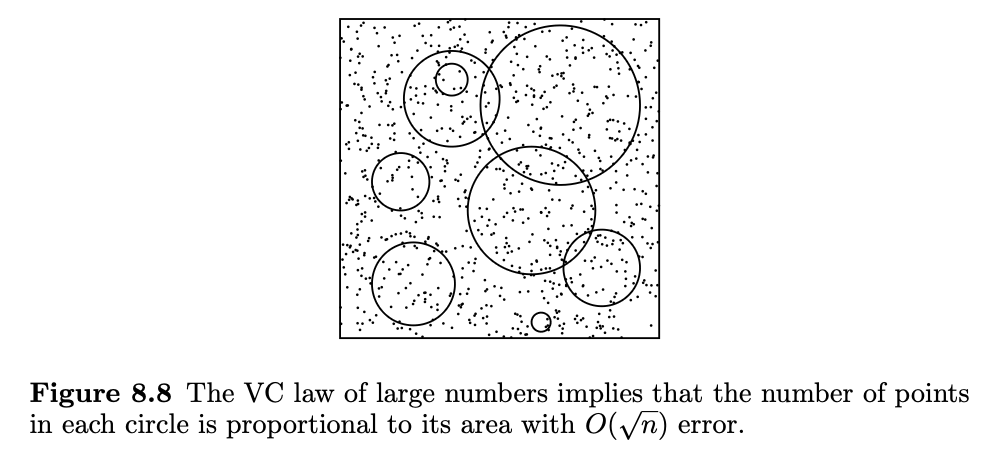
\includegraphics[width=0.8\textwidth]{Chapter 8/fig8-8.png}
\end{center}

Apply \cref{thm:8.3.15} for the class $\mathcal{F}$ of all indicator functions of circles in that square, which 
has VC dimension at most 3 (Exercise 8.13). Then, with high probability, the sample satisfies:
\[ \text{fraction of points in } \mathcal{C} = \mathrm{Area}(\mathcal{C}) + O(1 / \sqrt{n}) \]
simultaneously for all circles $\mathcal{C}$ in the square. This is a classic result in \textit{geometric 
discrepancy}, which also holds for half-planes, rectangles, polygons with few vertices, etc. - anything with 
finite VC dimension.
\end{example}

\begin{remark}[Uniform Glivenko-Cantelli classes]
\label{rmk:8.3.19}
A class of real-values functions $\mathcal{F}$ on a set $\Omega$ is called a \textit{uniform Glivenko-Cantelli} 
class if, for any $\varepsilon > 0$, 
\[ \lim_{n \to \infty} \sup_{\mu} P \left( \sup_{f \in \mathcal{F}} \left| \frac{1}{n} \sum_{i = 1}^{n} 
f(X_i) - \mathbb{E}\left[ f(X) \right] \right| > \varepsilon \right) = 0, \]
where the supremum is taken over all probability measures $\mu$ on $\Omega$, and where $X, X_1, \dots, X_n$ 
are i.i.d. points in $\Omega$ with distribution $\mu$. \cref{thm:8.3.15} followed by Markov's inequality implies 
that any Boolean class with finite VC dimension is uniform Glivenko-Cantelli. The converse is alse true 
(Exercise 8.27), so in fact the two are equivalent.
\end{remark}



% ----------8.4----------
\subsection{Application: Statistical Learning Theory}
Statistical learning (or machine learning) is about making predictions from data. Suppose there is an unknown 
function $T: \Omega \to \mathbb{R}$ on some set $\Omega$ (the \textit{target function}), and we get to see a 
few sample points $X_1, \dots, X_n$ drawn independently from some distribution on $\Omega$. Therefore, our 
\textit{training data} is 
\[ (X_i, T(X_i)), \ i = 1, \dots, n. \]
The goal is to use this sample to predict $T(X)$ for a new point $X$ drawn from the same distribution (See 
Figure 8.9).

\begin{center}
	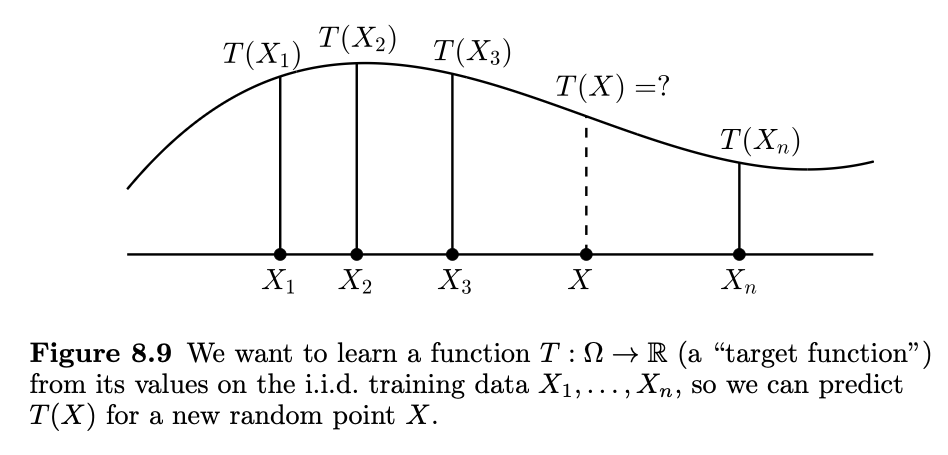
\includegraphics[width=0.8\textwidth]{Chapter 8/fig8-9.png}
\end{center}

\begin{example}[Classification]
\label{ex:8.4.1}
An important type of learning problems is classification, where the function $T$ is Boolean (takes value 0 and 
1), classifying points in $\Omega$ into two classes. For instance, imagine a health study with $n$ patients. 
For each patient, we record $d$ hralth parameters like blood pressure or temperature - that is our vector 
$X_i \in \mathbb{R}^d$. Suppose we also know if they have diabetes: $T(X_i) = 0$ (healthy) or $1$ (sick). The 
goal is to learn how to predict diabetes from data - that is, to learn the function $T: \mathbb{R}^d \to 
\{ 0, 1 \}$ so we can diagnose new patients based on their health parameters.
\end{example}


\subsubsection{Risk, Fit, and Complexity}
Given the training data, we want to find a function $f: \Omega \to \mathbb{R}$ that approximates $T$. 
We aim to minimize the \textit{risk}, defined as
\[ R(f) = \mathbb{E}\left[ (f(X) - T(X))^2 \right]. \]

\begin{example}[]
\label{ex:8.4.2}
In classification problems where $T$ and $f$ are boolean functions, the risk is the probability of 
misclassification:
\[ R(f) = P(f(X) \neq T(X)). \]
\end{example}

How much training data do we need? That depends on the complexity of the problem. If we believe the target 
function $T(X)$ behaves in a complicated way, we need more data. Since we usually don't know this up front, we 
limit our guesses $f$ to some class of functions $\mathcal{F}$, callled the \textit{hypothesis class}.

But how do we pick $\mathcal{F}$? There is no universal rule, but it should balance fit and complexity. If 
$\mathcal{F}$ is too simplistic - say, only linear functions - we might \textit{underfit} (Figure 8.10a) and 
miss real patterns. Too complex, we might \textit{overfit}, just memorizing the training data rather than 
generalizing from it (Figure 8.10b). The sweet spot is a hypothesis class that is just enough to capture the 
real patterns, without fitting the noise (Figure 8.10c).

\begin{center}
	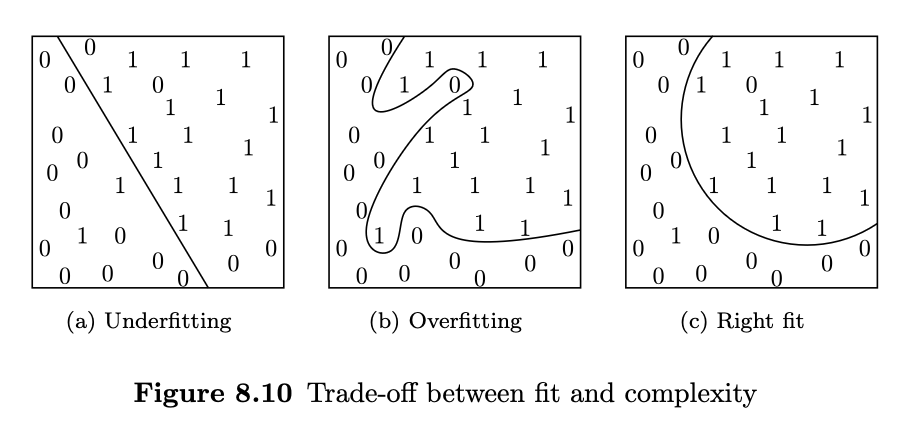
\includegraphics[width=0.8\textwidth]{Chapter 8/fig8-10}
\end{center}


\subsubsection{Empirical Risk Minimization}
Once we pick a hypothesis space $\mathcal{F}$, we might just choose the best function $f^*$ in it - one that 
minimizes the risk:
\[ f^* = \mathrm{arg}\min_{f \in \mathcal{F}} R(F). \]
The catch is that we can't actually compute $R(F)$ since we don't have access to the population $\Omega$. 
Solution? Use the training set and take the expectation.

\begin{definition}[]
\label{def:8.4.3}
For a function $f: \Omega \to \mathbb{R}$, define the \underline{empirical risk} and \underline{empirical 
minimizer} as 
\[ R_n(f) := \frac{1}{n}\sum_{i = 1}^{n}(f(X_i) - T(X_i))^2, \ f_n^* = \mathrm{arg}\min_{f \in \mathcal{F}} 
R_n(f). \]
\end{definition}

\begin{example}[Classification]
\label{ex:8.4.4}
In classification, where $f$ and $T$ take values 0 or 1, the empirical risk $R_n(f)$ is just the fraction of 
training points where $f$ gets it wrong: $f(X_i) \neq T(X_i)$. So empirical risk minimization picks the 
$f \in \mathcal{F}$ that makes the fewest mistakes on the training data.
\end{example}


\subsubsection{VC Generalization Bound}
Let's use the VC theory to bound the generalization error in any classification problem.

\begin{theorem}[VC generalization bound]
\label{thm:8.4.5}
Assume that the target $T$ is a Boolean function, and the hypothesis space $\mathcal{F}$ is a class of 
Boolean functions with finite VC dimension. Then 
\[ \mathbb{E}\left[ R(f_n^*) \right] \leq R(f^*) + C \sqrt{\frac{\mathrm{vc}(\mathcal{F})}{n}}. \]
\end{theorem}

\begin{proof}
\textbf{Step 1: Excess risk.} The following bound holds pointwise:
\[ R(f_n^*) - R(f^*) \leq 2 \sup_{f \in \mathcal{F}}|R_n(f) - R(f)|. \]
To check this, denote $\varepsilon := \sup_{f \in \mathcal{F}}|R_n(f) - R(f)|$ and write 
\begin{align*}
	R(f_n^*) 
	&\leq R_n(f_n^*) + \varepsilon \quad (\text{since } f_n^* \in \mathcal{F} \text{ by construction}) \\
	&\leq R_n(f^*) + \varepsilon \quad (\text{since } f_n^* \text{ minimizes } R_n \text{ in the class} 
	\mathcal{F}) \\
	&\leq R(f^*) + 2 \varepsilon \quad (\text{since } f^* \in \mathcal{F} \text{ by construction}).
\end{align*}
Subtracting $R(f^*)$ from both sides gives the claim.

\textbf{Step 2: Applying VC law of large numbers.} Thanks to the claim above, it is enough to show that 
\[ \mathbb{E}\left[ \sup_{f \in \mathcal{F}}|R_n(f) - R(f)| \right] \lesssim 
\sqrt{\frac{\mathrm{vc}(\mathcal{F})}{n}}. \]
Recalling the definitions of the empirical and population risk, we can rewrite the above as
\[ \mathbb{E}\left[ \sup_{\ell \in \mathcal{L}} \left| \frac{1}{n}\sum_{i = 1}^{n} \ell(X_i) 
- \mathbb{E}\left[ \ell(X) \right] \right| \right] \lesssim \sqrt{\frac{\mathrm{vc}(\mathcal{F})}{n}}, \]
where $\mathcal{L} = \{ (f - T)^2: \ f \in \mathcal{F} \}$. A moment's thought reveals that (Exercise 8.29) 
$\mathrm{vc}(\mathcal{L}) = \mathrm{vc}(\mathcal{F})$. Then, an application of \cref{thm:8.3.15} completes 
the proof.
\end{proof}

\begin{example}[Classification]
Say we have $n$ training data points $X_1, \dots, X_n$ sampled uniformly from the unit square (as in 
\cref{ex:8.3.18}), each labeled ``sick" (1) if it lies in some fixed circle $\mathcal{C}$, and ``healthy" 
otherwise. Our goal is to learn that ``sickness" circle $\mathcal{C}$ from the data. Let's do empirical risk 
minimization - pick a circle that best matches the labels, i.e. minimizes misclassifications.

How well do we do? Since the true circle $\mathcal{C}$ gives zero error, and the VC dimension of circles it 
at most 3 (Exercise 8.13), \cref{thm:8.4.5} tells us the risk for our learned circle is at most 
$O(1/\sqrt{n})$. So, new points can be classified just by checking if they are inside our learned circle - 
with misdiagnosis probability $O(1/\sqrt{n})$, which decreases as we get more data.
\end{example}

\begin{remark}[Bias-variance tradeoff]
\label{rmk:8.4.7}
The VC generalization bound (\cref{thm:8.4.5}) identifies two main sources of error in learning. The 
\textit{bias} term $F(f^*)$ comes from an imperfect choice of the hypothesis class (underfitting). We can 
shrink the bias by including more functions in $\mathcal{F}$ - ideally enough to capture the true target 
function $T$, making the bias equal zero. But then the \textit{variance} term 
$O(\sqrt{\mathrm{vc}(\mathcal{F})/n})$ grows. To keep it in check, we may use more training data (increase $n$) 
to avoid overfitting.
\end{remark}



% ----------8.5----------
\subsection{Generic Chaining}
Generic chaining improves the loose bound that Dudley's inequality can exhibit sometimes. It is essentially a 
technique of the chaining method we developed throughout the proof to Dudley's inequality (\cref{thm:8.1.4}).


\subsubsection{A Makeover of Dudley's Inequality}
Recall the bound we obtained by chaining in \cref{thm:8.1.4}:
\[ \mathbb{E}\left[ \sup_{t \in T}X_t \right] \lesssim \sum_{k = \kappa + 1}^{\infty} \varepsilon_{k - 1} 
\sqrt{\log_{}{|T_k|}}, \]
where $\varepsilon = 2^{-k}$, $T_k$ are smallest $\varepsilon$-nets of $T$ so $|T_k| = \mathcal{N}(T, d, 
\varepsilon_k)$, and $\kappa$ is chosen so that $|T_{\kappa}| = 1$.

Now, let's flip the approach: instead of fixing $\varepsilon_k$ and minimizing $|T_k|$, fix $|T_k|$ and 
minimize $\varepsilon_k$. Specifically, pick subsets $T_k \subset T$ such that 
\[ |T_0| = 1, \ |T_k| \leq 2^{2^k}, \ k = 1, 2, \dots \]
and define 
\[ \varepsilon_k = \sup_{t \in T} d(t, T_k) \]
where $d(t, T_k)$ denotes the distance from t to the set $T_k$ (the distance between a point $t$ and a set $A$ 
in a metric space is $d(t, A) = \inf_{} \{ d(t, a): \ a \in A \}$).

Each $T_k$ is then an $\varepsilon_k$-net, and the chaining bound becomes 
\[ \mathbb{E}\left[ \sup_{t \in T}X_t \right] \lesssim \sum_{k = 1}^{\infty} 2^{k/2} \sup_{t \in T} 
d(t, T_{k - 1}), \]
or after reindexing, 
\[ \mathbb{E}\left[ \sup_{t \in T}X_t \right] \lesssim \sum_{k = 0}^{\infty} 2^{k/2} \sup_{t \in T} d(t, T_k). \]


\subsubsection{The \texorpdfstring{$\gamma_2$}{} Functional and Generic Chaining}
So far, we have just restated Dudley's inequality in a new form - nothing major yet. The important step will 
come now. The generic chaining will allow us to pull the supremum \textit{outside} the sum above. The resulting 
quantity has a name:

\begin{definition}[]
\label{def:8.5.1}
Let $(T, d)$ be a metric space. A sequence of subsets $(T_k)_{k = 0}^{\infty}$ of $T$ satisfying 
\[ |T_0| = 1, \ |T_k| \leq 2^{2^k}, \ k = 1, 2, \dots \]
is called an \underline{admissible sequence}.

The \underline{$\gamma_2$ functional} of $T$ is defined as 
\[ \gamma_2(T, d) = \inf_{(T_k)} \sup_{t \in T} \sum_{k = 0}^{\infty} 2^{k / 2} d(t, T_k) \]
where the infimu is over all admissible sequences.
\end{definition}

The supremum in the $\gamma_2$ functional is outside the sum, hence it is smaller than the Dudley sum above. 
That might seem like a small change, but it can make a big difference in some cases (Exercise 8.34). Good news: 
we can improve Dudley's inequality (\cref{thm:8.1.4}) by replacing the Dudley sum (or integral) by the 
$\gamma_2$ functional:

\begin{theorem}[Generic chaining bound]
\label{thm:8.5.2}
Let $(X_t)_{t \in T}$ be a mean-zero random process on a metric space $(T, d)$ with subgaussian increments. Then 
\[ \mathbb{E}\left[ \sup_{t \in T}X_t \right] \leq CK \gamma_2(T, d). \]
\end{theorem}

\begin{proof}
We'll use the chaining method from the proof of Dudley's inequality, but more carefully.

\textbf{Step 1: Chaining setup.} As before, without loss of generality assume $K = 1$ and that $T$ is finite, 
which makes $\gamma_2(T, d)$ finite. Let $(T_k)$ be an admissible sequence of subsets of $T$ which almost 
attains the supremum in \cref{def:8.5.1}:
\[ \sup_{t \in T}\sum_{k = 0}^{\infty}2^{k/2}d(t, T_k) \leq 2 \gamma_2(T, d) < \infty. \]
Denote $T_0 = \{ t_0 \}$. There must be some $K$ for which $T_k = T$; otherwise some $t \in T$ would keep 
getting left out infinitely many sets $T_k$, so $d(t, T_k) > \varepsilon$ for all those $k$ and some fixed 
$\varepsilon > 0$, making the series above diverge.

We walk from $t_0$ to a general point $t \in T$ along the (finite) chain 
\[ t_0 = \pi_0(t) \to \pi_1(t) \to \pi_2(t) \to \cdot \to t \]
of points $\pi_k(t) \in T_k$ that are chosen as best approximations to $t$ in $T_k$, i.e.
\[ d(t, \pi_k(t)) = d(t, T_k). \]
Again, the displacement $X_t - X_{t_0}$ can be expressed as a telescoping sum:
\[ X_t - X_{t_0} = \sum_{k = 1}^{\infty}(X_{\pi_k(t)} - X_{\pi_{k - 1}(t)}). \]

\textbf{Step 2: Controlling the increments.} This is where we need to be more caredul. We would like that, with 
high probability, the following event holds:
\[ |X_{\pi_k(t)} - X_{\pi_{k - 1}(t)}| \lesssim 2^{k/2}d(t, T_k) \ \forall k \in \mathbb{N}, \forall t \in T. \]
Summing over all $k$ would lead to a desired bound in terms of $\gamma_2(T, d)$.

To prove the above, let's fix $k$ and $t$ first. The subgaussian assumption gives 
\[ \lVert X_{\pi_k(t)} - X_{\pi_{k - 1}(t)} \rVert_{\psi_2} \leq d(\pi_k(t), \pi_{k - 1}(t)). \]
So for every $u \geq 0$, the event 
\[ |X_{\pi_k(t)} - X_{\pi_{k - 1}(t)}| \leq Cu 2^{k/2} d(\pi_k(t), \pi_{k - 1}(t)) \quad (*) \]
holds with probability at least 
\[ 1 - 2 \exp{(-8u^2 2^k)}, \]
where we get the constant 8 by choosing $C$ to be big enough.

Now unfix $t \in T$ by taking a union bound over 
\[ |T_k| \cdot |T_{k - 1}| \leq |T_k|^2 \leq 2^{2^{k + 1}} \]
pairs $(\pi_k(t), \pi_{k - 1}(t))$. Also, unfix $k$ by taking a union bound over all $k \in \mathbb{N}$. Then 
$(*)$ holds simultaneously for all $t \in T$ and $k \in \mathbb{N}$ with probability at least 
\[ 1 - \sum_{k = 1}^{\infty} 2^{2^{k + 1}} \cdot 2 \exp{(-8u^2 2^k)} \geq 1 - 2 \exp{(-u^2)}. \]

\textbf{Step 3: Summing up the increments.} In the event that the bound $(*)$ does hold for all $t \in T$ and 
$k \in \mathbb{N}$, we can sum up the inequalities over $k \in \mathbb{N}$ and plug in the result into the 
chaining sum. We get 
\[ |X_t - X_{t_0}| \lesssim u \sum_{k = 1}^{\infty} 2^{k/2} d(\pi_k(t), \kappa_{k - 1}(t)) \quad (**), \]
where the notation $\lesssim$ hides an absolute constant factor. By the triangle inequality, 
\[ d(\pi_k(t), \pi_{k - 1}(t)) \leq d(\pi_k(t), t) + d(t, \pi_{k - 1}(t)). \]
Using that bound, reindexing, and plugging in the chaining bound from step 1, we get that the tright-hand side 
of $(**)$ is at most $Cu \gamma_2(T, d)$, that is 
\[ |X_t - X_{t_0}| \lesssim u \gamma_2(T, d). \]
Taking the supremum over $T$ yields 
\[ \sup_{t \in T}|X_t - X_{t_0}| \lesssim u \gamma_2(T, d). \]
Since this holds with probability at least $1 - 2 \exp{(-u^2)}$ for any $u > c$, we get 
\[ \left\lVert \sup_{t \in T}|X_t - X_{t_0}| \right\rVert_{\psi_2} \lesssim \gamma_2(T, d). \]
This quickly that the conclusion of \cref{thm:8.5.2}, and we're done.
\end{proof}

\begin{remark}[Generic chaining: supremum of increments]
\label{rmk:8.5.3}
Similarly to Dudley's inequality (\cref{rmk:8.1.5}), the generic chaining actually gives 
\[ \mathbb{E}\left[ \sup_{t, s \in T}|X_t - X_s| \right] \leq CK \gamma_2(T, d), \]
which is valid even without the mean zero assumption $\mathbb{E}\left[ X_t \right] = 0$.
\end{remark}

\begin{remark}[Generic chaining: a high-probability bound]
\label{rmk:8.5.4}
\cref{thm:8.5.2} gives only an expectation bound, but generic chaining actually gives a high-probability bound - 
we have aseen this before in \cref{rmk:8.1.6}.

Assuming $T$ is finite, for every $u \geq 0$, the event 
\[ \sup_{t, s \in T}|X_t - X_s| \leq CK \left[ \gamma_2(T, d) + u \cdot \mathrm{diam}(T) \right] \]
holds with probability at least $1 - 2 \exp{(-u^2)}$ (Exercise 8.35). For Gaussian processes, we can directly 
deduce this from Gaussian concentration.
\end{remark}


\subsubsection{Majorizing Measure and Comparison Theorems}
The $\gamma_2$ functional (\cref{def:8.5.1}) is usually harder to compute than covering numbers in Dudley's 
inequality. But it is often worth the effort - generic chaining is sharp up to constants:

\begin{theorem}[Talagrand majorizing measure theorem]
\label{thm:8.5.5}
Let $(X_t)_{t \in T}$ be a mean-zero Gaussian process on a set $T$, equipped with the canonical metric 
$d(t, s) = \lVert X_t - X_s \rVert_{L^2}$, as mentioned before. Then 
\[ c \gamma_2(T, d) \leq \mathbb{E}\left[ \sup_{t \in T}X_t \right] \leq C \gamma_2(T, d). \]
\end{theorem}

\begin{proof}
The upper bound directly comes from generic chaining (\cref{thm:8.5.2}). The lower bound is tricker hence not 
included in the text.
\end{proof}

The upper bound holds not just for Gaussian but also for all subgaussian processes. Therefore, by combining the 
upper and lower bounds, we can bound any subgaussian processes by the Gaussian one:

\begin{corollary}[Talagrand comparison inequality]
\label{cor:8.5.6}
Let $(X_t)_{t \in T}$ be a mean-zero random process on a set $T$ and let $(Y_t)_{t \in T}$ be a mean-zero 
Gaussian process. Assume 
\[ \lVert X_t - X_s \rVert_{\psi_2} \leq K \lVert Y_t - Y_s \rVert_{L^2} \text{ for all } t, s \in T. \]
Then 
\[ \mathbb{E}\left[ \sup_{t \in T}X_t \right] \leq CK \mathbb{E}\left[ \sup_{t \in T}Y_t \right]. \]
\end{corollary}

\begin{proof}
Consider the canonical metric $d(t, s) = \lVert Y_t - Y_s \rVert_{L^2}$ on $T$. Now just use the generic 
chaining bound (\cref{thm:8.5.2}) followed by the lower bound in the majorizing measure theorem 
(\cref{thm:8.5.5}) and we get 
\[ \mathbb{E}\left[ \sup_{t \in T}X_t \right] \lesssim K \gamma_2(T, d) \lesssim 
K \mathbb{E}\left[ \sup_{t \in T}Y_t \right]. \]
\end{proof}

\begin{remark}[Sudakov-Fernique]
\label{rmk:8.5.7}
\cref{cor:8.5.6} extends the Sudakov-Fernique inequality (\cref{thm:7.2.8}) to subgaussian processes - with 
only an absolute constant factor as the price for this generalization!
\end{remark}

We can also apply \cref{cor:8.5.6} for the canonical Gaussian process $Y_x = \left\langle g, x \right\rangle$ on 
a set $T \subset \mathbb{R}^n$, where $g \sim N(0, I_n)$. From section 7.5, 
\[ w(T) = \mathbb{E}\left[ \sup_{x \in T}\left\langle g, x \right\rangle \right] \]
is the \textit{Gaussian width} of the set $T$. We immediately get the following:

\begin{corollary}[Talagrand comparison inequality: geometric form]
\label{cor:8.5.8}
Let $(X_x)_{x \in T}$ be a mean-zero random process on a subset $T \subset \mathbb{R}^n$. Assume that 
\[ \lVert X_x - X_y \rVert_{\psi_2} \leq K \lVert x - y \rVert_{2} \text{ for all } x, y \in T. \]
Then 
\[ \mathbb{E}\left[ \sup_{x \in T}X_x \right] \leq CK w(T). \]
\end{corollary}

\begin{remark}[Subgaussian width & Gaussian width]
\label{rmk:8.5.9}
A nice consequence: if $X$ is a subgaussian random vector in $\mathbb{R}^n$, then 
\[ \mathbb{E}\left[ \sup_{t \in T}\left\langle X, t \right\rangle \right] \leq CKw(T) 
\text{ for any bounded set } T \subset \mathbb{R}^n, \]
where $K = \lVert X \rVert_{\psi_2}$. Just apply \cref{cor:8.5.8} to the process $(\left\langle X, x 
\right\rangle )_{x \in T}$, whose increments satisfy 
\[ \lVert \left\langle X, x \right\rangle - \left\langle X, y \right\rangle \rVert_{\psi_2} 
= \lVert \left\langle X, x - y \right\rangle \rVert_{\psi_2} \leq K \lVert x - y \rVert_{2} \]
by definition of a subgaussian random vector.
\end{remark}



% ----------8.6----------
\subsection{Chevet Inequality}
Talagrand's comparison inequality (generic chaining) is powerful and works in a wide range of settings. Let's 
use it on random quadratic forms: 
\[ \sup_{x \in T, y \in S} \left\langle Ax, y \right\rangle \leq ? \]
where $A$ is a random matrix and $T, S$ are bounded sets.

A special case where $T, S$ are Euclidean balls leads to the operator norm of $A$, which we did some analysis 
already (\cref{thm:4.4.3}). Here we go for a more general setting, and we'll just use two geometric quantities: 
the \textit{Gaussian width} $w(T)$, and the \textit{radius}, defined as 
\[ \mathrm{rad}(T) := \sup_{x \in T}\lVert x \rVert_{2}. \]

\begin{theorem}[Subgaussian Chevet's inequality]
\label{thm:8.6.1}
Let $A$ be an $m \times n$ random matrix with independent, mean-zero, subgaussian rows $A_i$. Let $T \subset 
\mathbb{R}^n$ and $S \subset \mathbb{R}^m$ be arbitrary bounded sets. Then 
\[ \mathbb{E}\left[ \sup_{x \in T, y \in S} \left\langle Ax, y \right\rangle \right] \leq 
CK [w(T) \mathrm{rad}(S) + w(S) \mathrm{rad}(T)] \]
where $K = \max_{i} \lVert A_i \rVert_{\psi_2}$. The same holds if ``rows" is replaced by ``columns".
\end{theorem}

\begin{proof}
We'll follow the proof for Theorem 7.3.1 (reference here) but with Talagrand's comparison inequality instead of 
Sudakov-Fernique's.

Without loss of generality, assume K = 1. We need to bound the random process 
\[ X_{uv}\left\langle Au, v \right\rangle, \ u \in T, v \in S. \]
To check that the increments are subgaussian, fix $(u, v), (w, z) \in T \times S$ and write 
\[ X_{uv} - X_{wz} = X_{uv} - X_{wv} + X_{wv} - X_{wz} = \left\langle A(u - w), v \right\rangle 
+ \left\langle Aw, v - z \right\rangle. \]
Using the triangle inequality and the subgaussian assumption (Exercise 3.34), we get 
\begin{align*}
	\lVert X_{uv} - X_{wz} \rVert_{\psi_2} 
	&\leq \lVert \left\langle A(u - w), v \right\rangle \rVert_{\psi_2} 
	+ \lVert \left\langle Aw, v - z \right\rangle \rVert_{\psi_2} \\
	&\lesssim \lVert u - w \rVert_{2}\lVert v \rVert_{2} + \lVert v - z \rVert_{2}\lVert w \rVert_{2} \\
	&\leq \lVert u - w \rVert_{2}\mathrm{rad}(S) + \lVert v - z \rVert_{2}\mathrm{rad}(T) \quad (*).
\end{align*}
Let's pick a simpler Gaussian process $(Y_{uv})$ for Talagrand's comparison inequality (\cref{cor:8.5.6}). The 
increment bound points us to a good choice:
\[ Y_{uv} := \left\langle g, u \right\rangle \mathrm{rad}(S) + \left\langle h, v \right\rangle 
\mathrm{rad}(T), \]
where $g \sim N(0, I_n)$ and $h \sim N(0, I_m)$ are independent. The increments of this process are 
\[ \lVert Y_{uv} - Y_{wz} \rVert_{L^2}^2 = \lVert u - w \rVert_{2}^2 \mathrm{rad}(S)^2 
+ \lVert v - z \rVert_{2}^2 \mathrm{rad}(T)^2. \]
Comparing this to the bound $(*)$, we find that 
\[ \lVert X_{uv} - X_{wz} \rVert_{\psi_2} \lesssim \lVert Y_{uv} - Y_{wz} \rVert_{L^2}, \]
where we used the inequality $a + b \leq \sqrt{2 (a^2 + b^2)}$. Applying Talagrand's comparison inequality 
(\cref{cor:8.5.6}), we finish the proof:
\begin{align*}
	\mathbb{E}\left[ \sup_{u \in T, v \in S}X_{uv} \right] 
	&\lesssim \mathbb{E}\left[ \sup_{u \in T, v \in S}Y_{uv} \right] \\
	&= \mathbb{E}\left[ \sup_{u \in T}\left\langle g, u \right\rangle \right] \mathrm{rad}(S) 
	+ \mathbb{E}\left[ \sup_{v \in S}\left\langle h, v \right\rangle \right] \mathrm{rad}(T) \\
	&= w(T) \mathrm{rad}(S) + w(S) \mathrm{rad}(T).
\end{align*}
\end{proof}

\begin{remark}[Operator norms of random matrices]
\label{rmk:8.6.2}
For the special case $T = S^{n - 1}, \ S = S^{m - 1}$, Chevet's inequality gives up the familiar sharp bound 
on the operator norm:
\[ \mathbb{E}\left[ \lVert A \rVert_{} \right] \leq CK (\sqrt{n} + \sqrt{m}), \]
which we proved earlier using $\varepsilon$-nets. But this new approach gives more flexibility! For example, 
picking $T, S$ as $\ell^p$ balls gives the $\lVert A \rVert_{p \to q}$ norm of a random matrix (Exercise 8.41).
\end{remark}

\begin{remark}[Gaussian Chevet inequality]
\label{rmk:8.6.3}
For Gaussian matrices $A$ with i.i.d. $N(0, 1)$ entries, we can even prove Chevet's inequality with sharp 
constant 1: 
\[ \mathbb{E}\left[ \sup_{x \in T, y \in S} \left\langle Ax, y \right\rangle \right] \leq 
w(T) \mathrm{rad}(S) + w(S) \mathrm{rad}(T), \]
and a reverse inequality up to a constant (Exercise 8.39). Later, we'll further improve Gaussian Chevet 
inequality in Section 9.7.1.
\end{remark}

